\documentclass[a4paper, twocolumn]{article}
\usepackage[utf8]{inputenc}
\usepackage{amsmath}
\usepackage{graphicx}
\graphicspath{documents/}
\usepackage{caption}
\captionsetup{font=scriptsize}
\usepackage[margin=0.5in]{geometry}

\title{Photoelectric Effect}
\author{
Garcia, Jorge A.\\
\and
Lane, Ryan C. \\
\and
Miller, Patrick C.
}
\date{February 21st, 2018\\\line(1,0){500}}

\begin{document}
\maketitle

\section{Purpose}
This experiment tested the postulate that light (photons) are quantized packets of energy $E=h\nu$.
It was this postulate that Einstein was able to extract from the mathematical equations of Max Planck the “Photoelectric Effect”.
Through this experiment the ratio of Planck's constant (h) to the charge of the electron (e) was able to be derived (h/e).
This analysis further demonstrates that the intensity of light is independent of photo-electron energy which clashes with
classical wave models that claim with increased intensity the amplitude of wavelength would increase as well.
Planck’s constant (h) has numerous implications and became the basis for the quantum mechanical sub-atomic world. 
After a few years Planck was awarded the Nobel prize for his theory of quantized light.

\section{Apparatus and Method}
\begin{itemize}
 \item PASCO (h/e) Apparatus: AP-9368 , AP-9369
 \item PASCO OS-9286A Mercury Vapor Light Source
\end{itemize}
The two main apparatus listed above face each other at the zero angle. The proper alignment of the two apparatus is paramount
for detecting the change in voltage as different angles cause diffraction lines of the incident light produced by the Mercury
apparatus to appear at the entrance window of the (h/e) apparatus. Located on the Mercury apparatus is a diffraction grating
that causes five distinct diffraction colors ultraviolet, violet, blue, green, and yellow to be incident on the (h/e) entrance
window at different angles. Located on the inside of the (h/e) apparatus is a parallel plate capacitor made of material that
allows a voltage change between the plates caused by the jumping of excited electrons. 

The kinetic energy of the electrons that jump is directly related to the frequency (energy) and angle of the incoming incident light and is one of the key measurements in the experiment.
There is a bit of work ($W_o$) done to get the electron from the positive plate to the negative plate so by applying a reverse potential between
the plates the stopping voltage is able to be determined. Max kinetic energy is then able to be extracted through measurement of the minimum
reverse potential needed to stop the photo-electrons.
\begin{align*}
 &KE_{max} = Ve \\
 \implies &h\nu = Ve + W_o \\
 \implies &V = (h/e)\nu - (o/e)
\end{align*}
Plotting the voltage (V) vs. the different frequencies of incident light we get a V-intercept $= (-W_o/e)$ and a slope $= (h/e)$

The next portion of measurements aims to prove the intensity of light is independent of photo-electron energy. By applying an
intensity filter at 5 different levels (.2 .4 .6 .8 100)\%  the incident light on two different distinct diffraction lines.
\begin{table}[h!]
 \centering
 \begin{tabular}{|c|c|c|}
  \hline
  \multicolumn{3}{|c|}{\textbf{Mercury Diffraction Lines}} \\
  \hline
  \textbf{Color} & \textbf{Frequency (Hz)} & \textbf{Wavelength (nm)} \\
  \hline
  Yellow & $5.187\times 10^{14}$ & 578.000 \\
  \hline
  Green & $5.490\times 10^{14}$ & 546.074 \\
  \hline
  Blue & $6.879\times 10^{14}$ & 435.835 \\
  \hline
  Violet & $7.409\times 10^{14}$ & 404.656 \\
  \hline
  Ultraviolet & $8.203\times 10^{14}$ & 365.483 \\
  \hline
 \end{tabular}
\end{table}

\section{Procedure}
Once properly aligned the incident light coming through the zero angle is essentially white light as observed on the (h/e) apparatus.
At discrete angles the diffraction lines of the incident light coming from the Mercury apparatus becomes apparent and at different
orders or pockets of distinct diffraction maxima. Due to the possible overlapping of the diffraction maxima measure the the first
and second order to obtain the best data.

The different diffraction lines are passed through the entrance window on the (h/e) apparatus which causes a change in stopping voltage. 
Trivially “zero out” the plate capacitors each time a new spectral line hits the entrance window of the (h/e) apparatus. 
For obvious reasons use filters when measuring the effects of lower energy diffraction lines (green and yellow)  in the event higher
energy photons are able to pass through the window and obscure the data.
Repeat process for all 5 distinct lines at both orders to achieve acceptable data.

Apply the intensity filter on two distinct lines and measure the stopping voltage to show that the intensity of light does
not effect the energy of the photo-electrons. Do this for all 5 levels of intensity and repeat for the second order lines.   

\section{Data and Uncertainties}
The first of the measurements done for the experiment was that of the stopping voltage for the different emission lines of Mercury from the left and
right, at both the first and second order. The stopping voltages for each color were then averaged, and their uncertainties determined. The error
in these measurements is probably from contamination of different energy photons in the first order lines, as well as change in incidence due to
alignment of the Mercury lamp. These results can be seen in Table \ref{table:stopvolt}.
\begin{table}[h!]
 \centering
 \begin{tabular}{|c|c|c|}
  \hline
  \multicolumn{3}{|c|}{\textbf{Photo-Electron Stopping Voltage}} \\
  \hline
  \textbf{Color} & \textbf{Avg Voltage $(V)$} & \textbf{Error $(V)$} \\
  \hline
  Yellow & 0.735 & 0.063 \\
  \hline
  Green & 0.815 & 0.046 \\
  \hline
  Blue & 1.404 & 0.034 \\
  \hline
  Violet & 1.641 & 0.023 \\
  \hline
  Ultraviolet & 1.892 & 0.054 \\
  \hline
 \end{tabular}
 \caption{Stopping voltage of different emission lines}
 \label{table:stopvolt}
\end{table}
\vfill\eject
In Table \ref{table:intdiff}, the stopping voltage for various intensities of two colors (Yellow and Blue) are displayed, as well as their respective
standard deviations.
\begin{table}[h!]
 \centering
 \begin{tabular}{|c|c|c|}
  \hline
  \multicolumn{3}{|c|}{\textbf{Intensity Differences}} \\
  \hline
  \textbf{Intensity \%} & \textbf{Yellow} & \textbf{Blue} \\
  \hline
  20\% & 0.727 & 1.440 \\
  \hline
  40\% & 0.739 & 1.459 \\
  \hline
  60\% & 0.746 & 1.463 \\
  \hline
  80\% & 0.750 & 1.465 \\
  \hline
  100\% & 0.750 & 1.462 \\
  \hline
  \hline
  \textbf{$\sigma$} & 0.009 & 0.009 \\
  \hline
 \end{tabular}
 \caption{Stopping voltage of Yellow and Blue at different intensities}
 \label{table:intdiff}
\end{table}

\section{Analysis and Uncertainties}
\subsection{Stopping Voltage of Wavelengths}
With the average stopping voltage and their respective uncertainties, determining Planck's constant
is a rather straightforward process. From the equation provided in the lab writeup:
\begin{equation} \label{eq:he}
 V = (h/e) \nu - (W_o/e)
\end{equation}
The expression $h/e$ would be the slope of Equation \ref{eq:he}. Planck's constant can the be calculated by:
\begin{equation*} \label{eq:planck}
 h = \frac{\Delta V}{\Delta \nu} e
\end{equation*}
With a known value for the elementary charge $e$ being $1.602\times 10^{-19}$ C.

The obtained voltages can be plotted against the frequencies of their respective emission lines, and with a
linear least squares fit, a value for $h/e$ is obtained from the slope of the fitted line. This implies
that the only propagation of the error from the measurements taken is in the error of the parameters of the
linear fit.
\begin{figure}[h!]
 \centering
 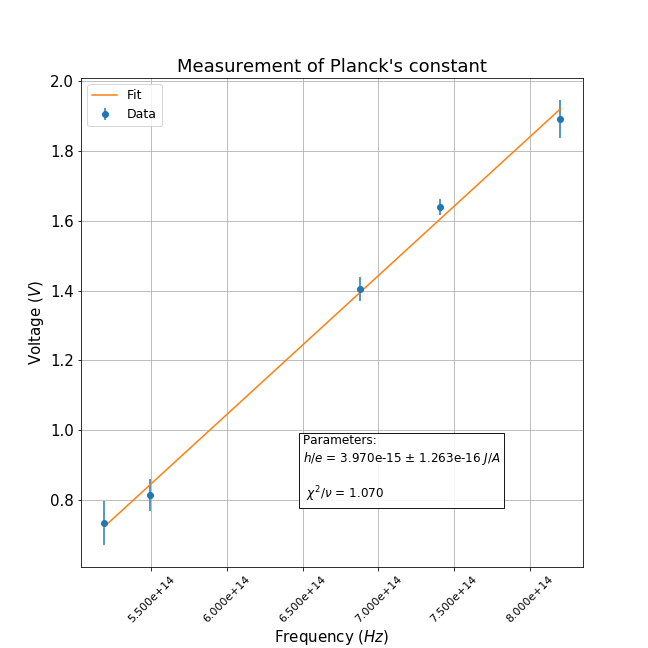
\includegraphics[scale = 0.4]{planck}
 \caption{Plot of frequency (Hz) against Voltage (V)}
 \label{fig:planck}
\end{figure}

The fit obtained is an excellent fit, as seen from the obtained Reduched Chi-Squared value. The determined value for
Planck's constant is then:
\begin{equation*}
h_{exp} = 6.359 \pm 0.202 \times 10^{-34} \text{$\frac{m^2 kg}{s}$}
\end{equation*}
\begin{equation*}
 \left|\frac{h_{exp}-h}{h}\right| = 4\%
\end{equation*}
\vfill\eject
\subsection{Intensity Differences}
From the lab writeup, it is known that the stopping voltage for each wavelength should be independent of the intensity of the light; it only
depends on the energy of the incidental photons. As can be seen from the measurements in Table \ref{table:intdiff}, there is not much
of a variance between the values, but it can be consistently be seen that at higher intensities, the stopping voltage is higher. This
is most likely due to instrumental reasons, as lowering the intensity may cause a slight shift in the wavelength of the emission line.

\section{Results}
The results show a linear positive slope between the stopping voltage and frequency. Taking the average
of both orders and their effects on the stopping voltage gave an accurate account of the $h/e$ measurements.
Obviously background radiation, high energy photons from the incident light, and possible alignment
issues (human error) skewed the data and were suspect in determining the error of our measurements. We
achieved an $h/e$ value of $3.970 \pm 0.1263 \times 10^{-15}$, which is within 4\% of $h/e$ actual. What was perhaps
more interesting was the almost non-existent deviation the intensity caused on the stopping voltage. At a
mere 0.009\% deviation from our measured values in the first experiment classical wave theory has been
further diminished analytically.

\section{Conclusions}
We successfully carried out all tasks that were assigned and with relatively low uncertainty of the
measured values. The accuracy of our measurement of $h/e$ is the biggest takeaway in this experiment and
the low deviation of our second experiment values is the cherry on top. In one experiment we set
ourselves up for the measurement of Planck’s constant (h) and provided evidence against a classical
theory and strengthened the theory of the photoelectric effect.

\end{document}